\chapter{Einführende Flugtests: Misson-Mode}
Einführend wird die Verwendung von Bodenstation und Drohne im Missionsmodus beschrieben. Zum Einsatz kommt die Software \textit{QGroundcontrol} auf dem PC. 

\begin{multicols}{2}
    Der Missionsplaner kann jederzeit oben Links in \textit{QGroundcontrol}, wie in Bild \ref{fig:qgc_mission_plan} dargestellt, aufgerufen werden. Es öffnet sich ein erweitertes Menü. Nach dem Anlegen des jeweiligen Planes muss dieser zur Drohne hochgeladen werden (nur während eine Verbindung hergestellt ist). Anschließend kann der Missions-Planer verlassen und die jeweilige Mission über das wechseln in den Mission-Mode gestartet werden.
    \vfill\null
    \columnbreak
    \begin{figure}[H]
        \centering
        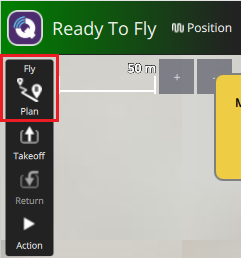
\includegraphics[width=0.4\textwidth]{images/mission_plan_open.png}
        \caption[QGroundControl Missionplaner-Menu]{QGroundControl Missionplaner-Menu wird durch Klick auf Rot umrahmten Button geöffnet}
        \label{fig:qgc_mission_plan}
    \end{figure}
\end{multicols}

\newpage
\section{Flug auf gerade Linie}
Für den einfachsten Fall lassen sich im Missionsplaner eine Liste von Wegpunkten anlegen, siehe dazu Bild \ref{fig:qgc_mission_plan_wp}. Nachdem am linken Rand \enquote{Waypoint} ausgewählt wurde lassen sich diese beliebig auf der Karte platzieren. Der erste Punkt beschreibt den Start, der letzte kann als Landepunkt dienen. Andernfalls kann die Drohne zum Startpunkt zurückkehren oder in letzter Position stehen bleiben.\\
Jeder Wegpunkt beschreibt eine Position im Raum. Die Parameter Höhe, Bewegungsgeschwindigkeit und eine relative Drehung zur Vorwärtsrichtung (Yaw) können für jeden Punkt separat am rechten Rand festgelegt werden.\\
Im unteren Bildbereich ist das Höhenprofil über den Weg eingezeichnet: in Orange gefärbt die jeweilige Flughöhe der Drohne, in Grün der Boden laut \gls{gps} Karte.\\
Mit den im Bild gezeigten Einstellungen wird die Drohne starten, auf gerade Linie nach vorn fliegen und anschließend landen. Dieses Verhalten wurde in der Simulation überprüft. Dazu wurde ein Hilfsprogramm geschrieben, welches die derzeitige Geschwindigkeit, Höhe und Orientierung der Drohne mitschreibt. Eine Auswertung als Diagramm ist zu sehen in Bild \ref{fig:qgc_mission_plan_wp_dia}.

\begin{figure}[h]
    \centering
    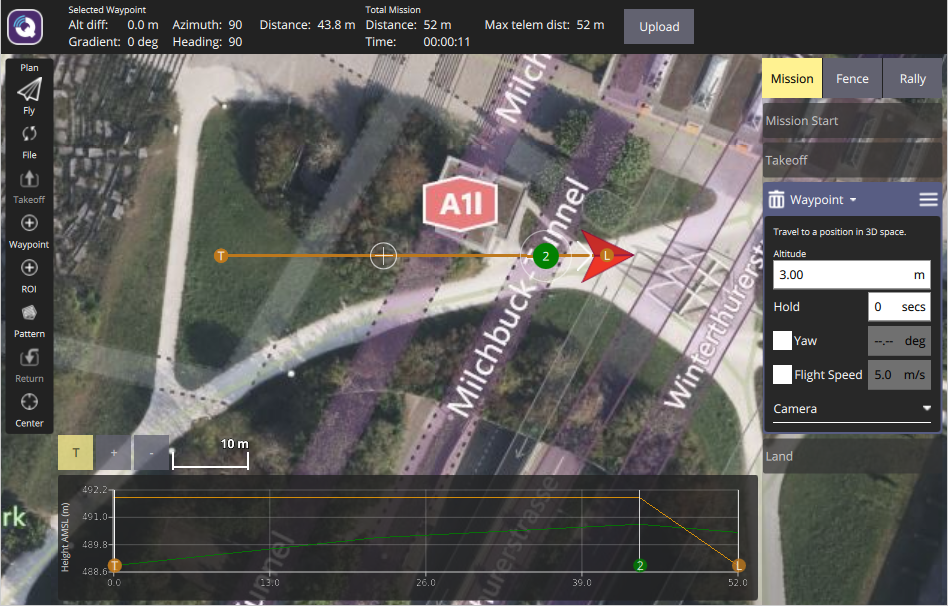
\includegraphics[width=0.6\textwidth]{images/mission_plan_mission.png}
    \caption[QGroundControl Missionplaner-Wegpunkte]{QGroundControl Missionplaner-Wegpunkte}
    \label{fig:qgc_mission_plan_wp}
\end{figure}

\begin{figure}[h]
    \centering
    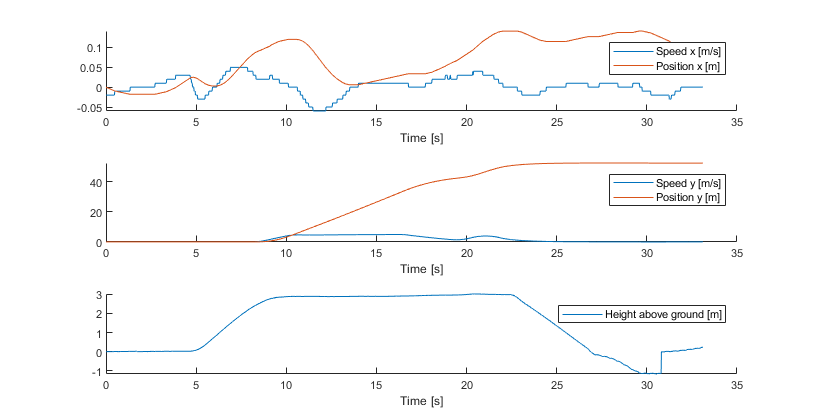
\includegraphics[width=0.9\textwidth]{images/mission_plan_mission_dia.png}
    \caption[Auswertung Missionsplaner-Wegpunkte]{Auswertung Missionsplaner-Wegpunkte: Diagramme geplottet von Matlab. In den oberen Diagrammen zu sehen sind die jeweilige x-/y-Geschwindigkeit und -Position während des Fluges. Positive x-Richtung zeigt nach Norden, positive y-Richtung nach Osten. Im unteren Diagramm die Flughöhe. Da der Simulator von einer flachen Welt ausging, die GPS-Karte aber eine Position in Östterreich annahm, wurde der Landepunkt tiefer als der eigentliche Boden berechnet. Die Drohne konnte diesen Fehler beim Landen bei ca. $30s$ ausgleichen und blieb sicher stehen.}
    \label{fig:qgc_mission_plan_wp_dia}
\end{figure}

\section{Rally-Kartierung}

\section{Flug mit GeoFence}

\section{Flug mit ROI}

\section{Zusammenfassung}


